\chapter{Hybrid Model Persistence}
\label{ch:hybrid_model_persistence}

Reconstructing the state of a change-based model by replaying its editing history every time the model needs to be queried or modified can get increasingly expensive as the model grows in size. In Chapter \ref{ch:optimised_loading}, this work has proposed a method to speed up the reconstruction by not replaying change events that do not have any effect to the eventual states of a model. However, the method is by far still outperformed by loading a model directly from its state-based persistence. Thus, as another solution, this work integrates change-based and state-based model persistence mechanisms in a hybrid model persistence approach that delivers the best of both worlds. This Chapter presents the design of the hybrid model persistence approach and report on its impact on time and memory footprint for model loading, saving, and storage space usage.

\section{Introduction}
\label{sec:introduction_5}
Saving models in change-based persistence (CBP) comes at the cost of ever-growing model files \cite{DBLP:conf/edoc/KoegelHLHD10,DBLP:journals/entcs/RobbesL07} since all changes (even deleting model elements) are recorded in an editing log, which naturally leads to longer loading times \cite{mens2002state}. 
In Chapter \ref{ch:optimised_loading}, this work has proposed a method to speed up the reconstruction by not replaying change events that do not have any effect to the eventual states of a model. However, the method is by far still outperformed by loading a model directly from its state-based persistence.
Thus, this chapter proposes another solution to address the issue by introducing the concept of hybrid persistence of models. In hybrid model persistence the change-based representation is augmented with a state-based representation (which may be derived from the change-based representation) of the latest state of the model which is used to speed up model loading and querying.

This Chapter is structured as follows. Section \ref{sec:change_and_state_based_model_persistence} introduces the concept of change-based model persistence and recent work on state-based model persistence. Sections \ref{sec:hybrid_model_persistence} and \ref{sec:implementation} present the proposed approach to hybrid model persistence and its implementation. Sections \ref{sec:evaluation_5} and \ref{sec:discussion_5} present and discuss experimental results and evaluation. Section \ref{sec:conclusions_5} concludes this Chapter.

\section{Comparing Change and State-based Model Persistence}
\label{sec:change_and_state_based_model_persistence}
Table \ref{table:persistence_comparsion} summarises the benefits (+) and drawbacks (-) of change and state-based model persistence. To load a state-based model, only the elements that exist in the final state need to be loaded into memory. To load a change-based persistence model, all the events that lead to the final state must be replayed to load the model in memory. Loading times for state-based models are proportional to the size of the model. Loading times for change-based models are proportional to the number of events. As a result, loading times of change-based models will always increase over time and are considerably longer than for state-based model persistence \cite{yohannis2018towards,mens2002state}. 

\begin{table}[ht]
  \caption{Comparison of model persistence approaches.}
  \label{table:persistence_comparsion}
  \centering
  \begin{small}
    \begin{tabular}{ c c c c }
      \hline 
      \textbf{Dimensions} & \textbf{Change-based} & \textbf{State-based} \\
      \hline 
      Load Time & $-$ & $+$ \\
      Save Time & $+$ & $-$ \\
%      Comparison Time & $+$ & $-$ \\
      Storage & $-$ & $+$ \\
      \hline 
    \end{tabular}
  \end{small}
\end{table}

To store an state-based model, all the elements that exist in the final state must be persisted. To save a change-based model, only the change events in the last session need to be persisted. Storing times of state-based models are proportional to the size of the model. Storing times of change-based models are proportional to the number of events in a session. As a result, storing times of change-based models can be considerably shorter than for state-based models \cite{yohannis2018towards}. Comparing and finding the differences between two versions of a state-based model is expensive \cite{Kolovos:2009:DMM:1564596.1564641} ($O(N^2)$ in the general case) which affects the efficiency of change visualisation and comprehension, and has a substantial impact on downstream activities such as incremental model transformation \cite{DBLP:conf/ecmdafa/OgunyomiRK15} and validation.

%By contrast, in change-based model persistence, changes are first-class entities in the persisted model file and as such, model comparison and differencing is relatively inexpensive. 
The main downsides of change-based model persistence are it's model file sizes \cite{DBLP:journals/entcs/RobbesL07,DBLP:conf/edoc/KoegelHLHD10} and ever-increasing loading times \cite{mens2002state}. Loading times can be reduced by around 50\% by processing the changelog, detecting, memorising and subsequently ignoring change events that have no impact to the final state of the model. The loading times are still substantially longer -- more than 6.4 times slower and even longer as the persisted changes increase -- than loading times for state-based approaches \cite{yohannis2018towards}. 

\section{Hybrid Model Persistence}
\label{sec:hybrid_model_persistence}
To achieve the best of both worlds, this work introduces a hybrid model persistence approach which combines change-based and state-based model persistence, to work together side-by-side. An overview of the proposed approach is illustrated in Fig. \ref{fig:hybrid_persistence}. In the proposed approach a \textit{hybrid} model is stored in two representations at the same time: a change-based (e.g. using EMF CBP \cite{epsilonlabs2019emfcbp} and a state-based representation (e.g. using XMI \cite{omg2018xmi} or a database-backed approach such as NeoEMF \cite{daniel2016neoemf}). The change-based representation is perceived as the main representation of a model, while the state-based representation can be fully derived from the change-based representation.

\begin{figure}[t]
  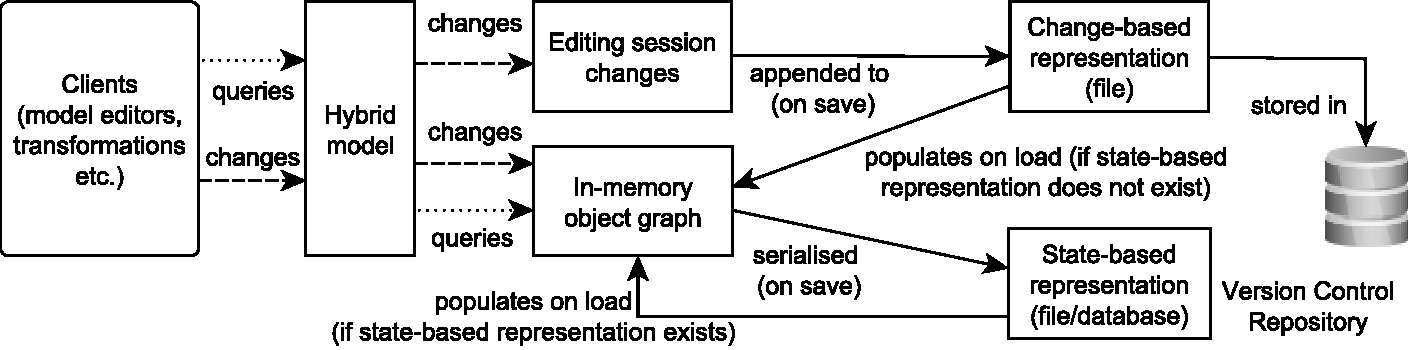
\includegraphics[width=\linewidth]{images/hybrid_persistence}
  \captionof{figure}{The mechanism of hybrid model persistence.}
  \label{fig:hybrid_persistence}
\end{figure}

\textbf{Loading a hybrid model.} Models are loaded into in-memory object graphs that clients (e.g. editors, transformations) can then interact with; depending on the state persistence mechanism, the object graph may be loaded in its entirety at startup (e.g. XMI) or loaded progressively, in a lazy manner (e.g. NeoEMF/CDO \cite{daniel2016neoemf,eclipse2019cdo}. In the proposed hybrid approach, if the state-based counterpart already exists, the in-memory object graph is populated from it; otherwise, it is populated by replaying the complete editing history recorded in the change-based representation.

\textbf{Changing a hybrid model.} When an element in a loaded model is created, modified or deleted, the change is applied to the in-memory object graph and is also recorded in an in-memory list of changes (\textit{Editing session changes} in Fig 2). This work uses the term \emph{editing session} for the period between loading a model and saving back to disk. 

\textbf{Saving a hybrid model.} The current version of the in-memory object graph is stored in the preferred state-based representation. The list of changes recorded in the current editing session (with optional processing, as described above) is appended to the change-based representation.

\textbf{Versioning a hybrid model.} Since the state-based representation is fully derived from the change-based representation, if a model needs to be versioned (e.g. in a Git repository), only the change-based representation needs to be stored. The first time it is loaded after being checked out/cloned, the state-based representation is computed and persisted locally and is used in subsequent model loading steps.

\textbf{Comparing hybrid models.} To compare two hybrid models -- discussed in Chapters \ref{ch:model_differencing} and \ref{ch:conflict_detection}, their change-based representations are used: this is much more efficient than state-based comparison. 

\section{Implementation}
\label{sec:implementation}
This work has implemented the proposed hybrid model persistence approach in a prototype \cite{epsilonlabs2019emfcbp} on top of the Eclipse Modeling Framework (EMF) \cite{steinberg2008emf}. The prototype makes use of an existing implementation of change-based model persistence, the EMF CBP \cite{DBLP:conf/models/YohannisKP17}, augmented with two state-based model persistence implementations: NeoEMF \cite{daniel2016neoemf} and XMI \cite{omg2018xmi}.

\begin{landscape}
\begin{figure}[]
  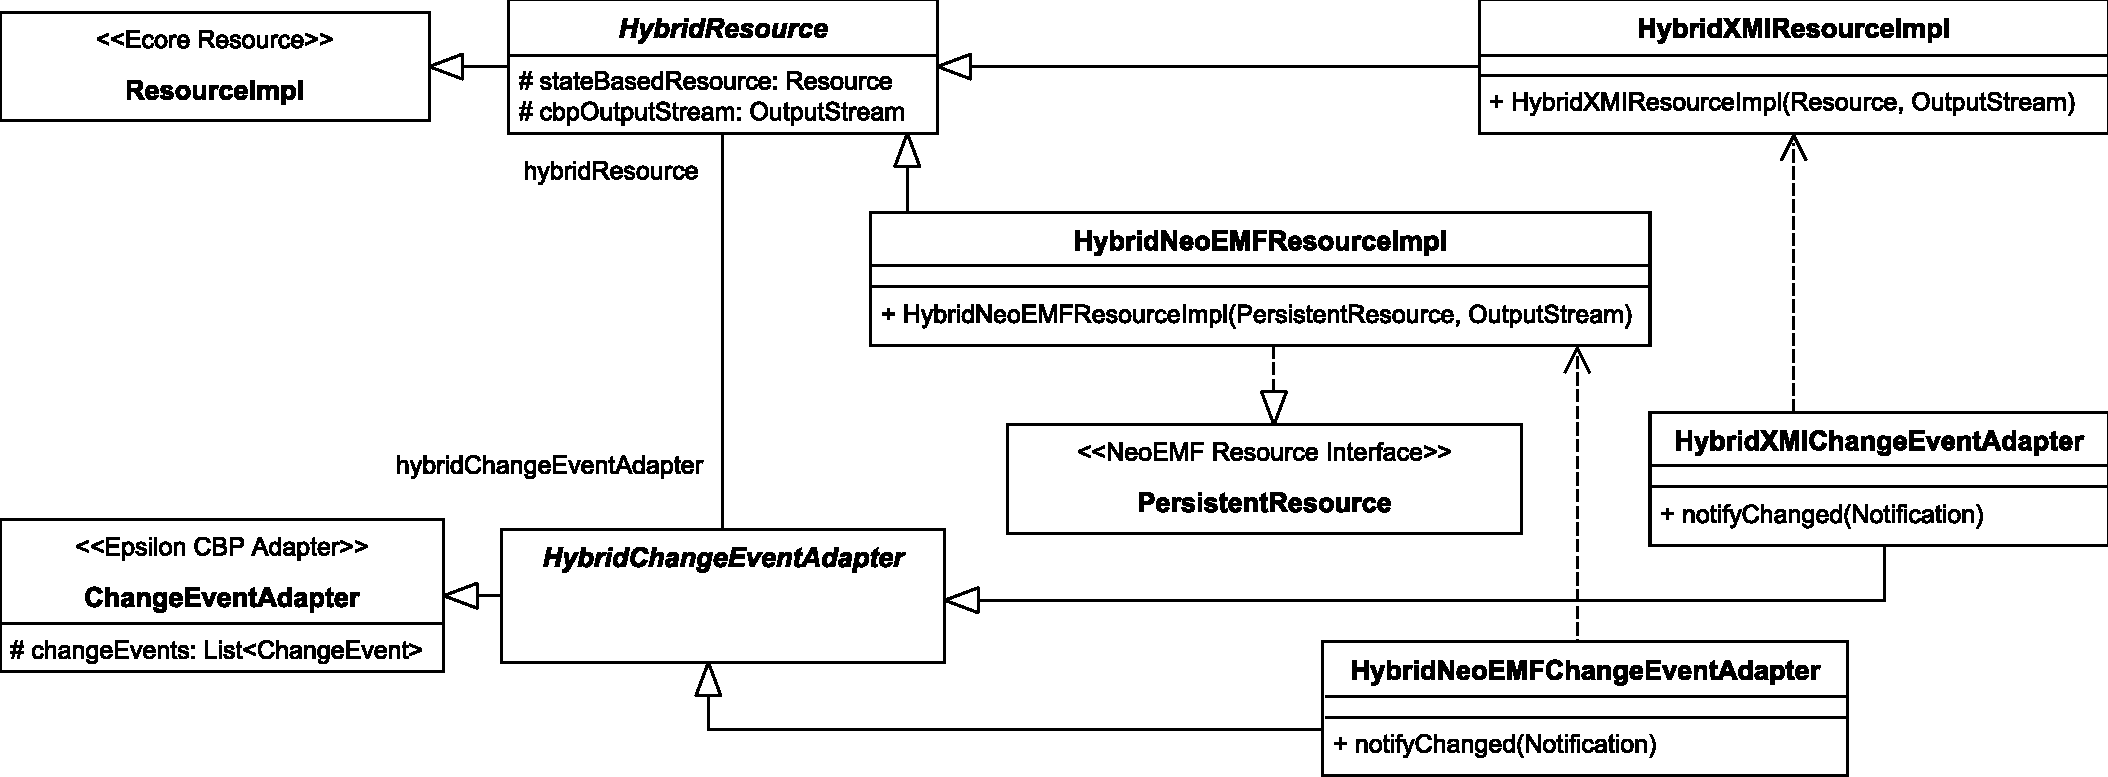
\includegraphics[width=\linewidth]{images/class_diagram}
  \captionof{figure}{Class diagram showing the core components of the hybrid model persistence implementation.}
  \label{fig:class_diagram}
\end{figure}
\end{landscape}

XMI has been selected as a standard state-based model persistence format (natively supported by EMF), and NeoEMF as a best-of-breed representative of database-backed state-based model persistence frameworks. The core components of the prototype are presented in Fig. \ref{fig:class_diagram}. 

The EMF CBP provides a \textsf{ChangeEventAdapter} class \cite{DBLP:conf/models/YohannisKP17} that extends from Ecore's \textsf{EContentAdapter} adapter class \cite{eclipse2018eContentAdapter}
. This class collects changes made to the in-memory object graph of an EMF model in the form of a list of events \textsf{changeEvents}. Based on this class, this work derived an adapter class, \textsf{HybridChangeEventAdapter}, for the hybrid model persistence implementation. It is an abstract class so that it can be further derived to create different implementations of adapter classes for different types of state-based model persistence. The \textsf{HybridNeoEMFChangeEventAdapater} is the adapter class for NeoEMF, and the \textsf{HybridXMIChangeEventAdapater} for XMI. These classes override \textsf{notifyChanged}(\textsf{Notification}) in the \textsf{ChangeEventAdapter} class, to handle events that are specific to NeoEMF and XMI, respectively.

This work also created a resource class for hybrid persistence, \textsf{HybridResource} (a resource class is a class dedicated to interacting with a persistence, e.g. save, load, get contents), derived from the Ecore's \textsf{ResourceImpl} \cite{eclipse2018resourceImpl}
. The class is again abstract so that it can be realised in different resource implementation classes for different state-based model persistence. The \textsf{HybridResource} class contains the \textsf{stateBasedResource} field which is used to refer to a state-based model persistence that is being used, and the \textsf{cbpOutputStream} field that refers to an \textsf{OutputStream} (e.g. file, in-memory) as the representation of the change-based model persistence for saving changes. \textsf{HybridResource} has an association with \textsf{HybridChangeEventAdapater}, so that the former can access the events collected by the latter, and the latter can also use facilities provided by the former (e.g. getting the identity of an element in the resource; saving changes to a change-based model representation).

The resource implementation classes for NeoEMF and XMI are \textsf{HybridNeoEMFResourceImpl} and \textsf{HybridXMIResourceImpl} respectively. \textsf{HybridNeoEMFResourceImpl} also implements the NeoEMF's \textsf{PersistenceResource} interface \cite{atlanmod2018persistentResource}
so that specific NeoEMF's methods can be used (e.g. \textsf{close}(), to close a connection with a backend database).

\section{Evaluation}
\label{sec:evaluation_5}
In this section, this work compares hybrid model persistence (EMF CBP with each of NeoEMF and XMI) vs state-based model persistence (NeoEMF or XMI only) on storage space usage, loading and saving time and memory footprint, and demonstrate that hybrid model persistence can still perform fast model loading and saving. 

The evaluation was performed on Intel\textsuperscript{\textregistered} Core\textsuperscript{TM} i7-6500U CPU @ 2.50GHz 2.59GHz, 12GB RAM, and the Java\textsuperscript{TM} SE Runtime Environment (build 1.8.0 \textunderscore162-b12). For the evaluation, this work used models reverse-engineered from the Java source code of the Epsilon \cite{eclipse2017epsilon,eclipse2018epsilongit} and BPMN2 \cite{eclipse2017bpmn2} projects. For state-based representation of the models, this work used the MoDisco tool \cite{DBLP:journals/infsof/BruneliereCDM14} to generate XMI-based UML2 \cite{eclipse2017uml2} models that reflect the classes, fields, and operation signatures of the source code of the project and then imported the generated models into NeoEMF. This work also derived MoDiscoXML models \cite{eclipse2018modiscoxml} from the Wikipedia article on the United States \cite{wikipedia2018us}. This work then used reverse-engineering to generate a change-based model persistence for each project based on the differences between consecutive versions of the models.

\begin{table}[ht]
\centering
\begin{footnotesize}
\caption{Space usage for the Epsilon and BPMN2 projects, 
and the Wikipedia's United States article (m = million events, MB = Megabytes, KB = Kilobytes).}
\label{table:space_usage}
\begin{tabular}{| c | c |  c  c c  c  c |}
\hline 
\textbf{Case} & \textbf{\makecell{Generated\\From}} & \textbf{\makecell{Type}} &
\textbf{\makecell{Element\\Count}} & \textbf{\makecell{Event\\Count}} & \textbf{\makecell{Space\\Size}} & \textbf{\makecell{Average\\Space\\Size}}
\\
\hline
%----

\multirow[c]{5}{*}{Epsilon} & \multirow[b]{3}{*}{\makecell{940\\commits}} & XMI & 88,020 & --- &
\makecell{9.44\\MBs} & \makecell{112 bytes/\\element} \\
\hhline{~~-----} 
& & NeoEMF & 88,020 & --- &
\makecell{188\\MBs} & \makecell{2 KBs/\\element} \\
\hhline{~~-----} 
& & \makecell{Epsilon\\CBP} & --- & 4.3 m & \makecell{406\\MBs} & \makecell{98 bytes/\\change event} \\
\hline
%----

\multirow[c]{5}{*}{BPMN2} & \multirow[b]{3}{*}{\makecell{192\\commits}} & XMI & 62,062 & --- & \makecell{6.55\\MBs} & \makecell{110 bytes/\\element} \\
\hhline{~~-----} 
& & NeoEMF & 62,062 & --- &
\makecell{134\\MBs} & \makecell{2 KBs/\\element} \\
\hhline{~~-----} 
& & \makecell{Epsilon\\CBP} & --- & 1.2 m & \makecell{109\\MBs} & \makecell{92 bytes/\\change event} \\
\hline
%----

\multirow[c]{5}{*}{Wikipedia} & \multirow[b]{3}{*}{\makecell{10,187\\versions}} & XMI & 13,112 & --- & \makecell{1.28\\MBs} & \makecell{102 bytes/\\element} \\
\hhline{~~-----} 
& & NeoEMF & 13,112 & --- &
\makecell{31.8\\MBs} & \makecell{2 KBs/\\element} \\
\hhline{~~-----} 
& & \makecell{Epsilon\\CBP} & --- & 62.3 m & \makecell{5.85\\GBs} & \makecell{98 bytes/\\change event} \\
\hline
\end{tabular}
\end{footnotesize}
\end{table}

\subsection{Storage Space Usage}
\label{sec:storage_space_usage}
For the Epsilon project, this work has successfully generated a change-based model persistence from version 1 up to version 940 and also change-based model persistence for the BPMN2 project and Wikipedia article up to version number 192 and 10,187 respectively. The details (element count, event count, space size, and average space size per element or event) of their models, when persisted in XMI, NeoEMF, and EMF CBP are shown in Table \ref{table:space_usage}. The last column of the table derives an average space usage per element (for the state-based model persistence) or event (for the change-based model persistence). Thus, we can estimate the storage space usage for a hybrid model persistence to be the combination of change-based model persistence and the appropriate state-based model persistence space usage.

\subsection{Time and Memory Footprint of Loading and Saving Models}
\label{sec:model_loading_time}
This work evaluated the performance of our hybrid persistence prototype against XMI and NeoEMF regarding time and memory footprint for loading and saving. In the evaluation, experiments were repeated 22 times for each dimension measured. Since the data were not normally distributed, this work used the nonparametric Mann-Whitney U test \cite{doi:10.1002/9780470479216.corpsy0524} with 5\% significance level.

  \begin{table}
    \centering
    \begin{footnotesize}
      \caption{The comparison on time and memory footprint for loading and saving models of the hybrid and state-based-only persistence. The time is in seconds, and the memory footprint is in MBs.}
      \label{table:time_memory_footprint}
      \begin{tabular}{ | c | c | c | c | c | c | c | c | c | }
        \hline
        \multirow{2}{*}{\textbf{\makecell{Dimen\\sion}}} & \multirow{2}{*}{\textbf{Case}} & \multirow{2}{*}{\textbf{Backend}} & \multicolumn{2}{c|}{\textbf{Hybrid}} & \multicolumn{2}{c|}{\textbf{State-based}} & \multicolumn{2}{c|}{\textbf{Significance}} \\
        \hhline{~~~------}
        & & & $mean$ & $sd$ & $mean$ & $sd$ &  $W$ & $p$-$value$ \\
        \hline
        %----------------
        \multirow[c]{6}{*}{\makecell{Loading\\Time}} & \multirow{2}{*}{Epsilon} & NeoEMF & 0.292 & 0.061 & 0.279 & 0.023 & 258 & \textbf{0.72}\\ 
        \hhline{~~-------}
        & & XMI & 0.317 & 0.006 & 0.270 & 0.018 & 26 & $<$ 0.05 \\
        \hhline{~--------}
        &\multirow{2}{*}{BPMN2} & NeoEMF & 0.308 & 0.071 &0.286 & 0.025 & 230 & \textbf{0.79}\\ 
        \hhline{~~-------}
        & & XMI & 0.212 & 0.016 & 0.179 & 0.016 & 37 & $<$ 0.05 \\
        \hhline{~--------}
        &\multirow{2}{*}{Wikipedia}  & NeoEMF & 0.262 & 0.048 & 0.273 & 0.062 & 250 & \textbf{0.86}\\ 
        \hhline{~~-------}
        & & XMI & 0.045 & 0.001 & 0.040 & 0.001 & 0 & $<$ 0.05 \\
        \hline
        \hline
        %--------------------
        
        \multirow[c]{6}{*}{\makecell{Saving\\Time}} & \multirow{2}{*}{Epsilon} & NeoEMF & 0.0892 & 0.0421 & 0.0829 & 0.0494 & 216 & \textbf{0.55}\\ 
        \hhline{~~-------}
        & & XMI & 0.411 & 0.023 & 0.397 & 0.015 & 78 & $<$ 0.05 \\
        \hhline{~--------}
        &\multirow{2}{*}{BPMN2} & NeoEMF & 0.0777 & 0.0424 & 0.0775 & 0.0452 & 213 & \textbf{0.51}\\ 
        \hhline{~~-------}
        & & XMI & 0.33 & 0.007 & 0.28 & 008 & 0 & $<$ 0.05 \\
        \hhline{~--------}
        &\multirow{2}{*}{Wikipedia} & NeoEMF & 0.135 & 0.048 & 0.120 & 0.024 & 218 & \textbf{0.59}\\ 
        \hhline{~~-------}
        & & XMI & 0.024 & 0.048 & 0.020 & 0.002 & 42 & $<$ 0.05 \\
        \hline
        \hline
        %--------------------
        
        \multirow[c]{6}{*}{\makecell{Loading\\Memory\\Footprint}} & \multirow{2}{*}{Epsilon} & NeoEMF & 38.601 & 0.878 & 10.014 & 1.088 & 0 & $<$ 0.05\\ 
        \hhline{~~-------}
        & & XMI & 10.72018 & 0.00022 & 10.72009 & 0.00024 & 0 & $<$ 0.05 \\
        \hhline{~--------}
        &\multirow{2}{*}{BPMN2} & NeoEMF & 40.78 & 1.29 & 27.20 & 1.05 & 0 & $<$ 0.05\\ 
        \hhline{~~-------}
        & & XMI & 6.73367 & 1.29305 & 6.73367 & 0.00056 & 101 & $<$ 0.05 \\
        \hhline{~--------}
        &\multirow{2}{*}{Wikipedia}  & NeoEMF & 35.91 & 1.03 & 27.25 & 0.54 & 27.25 & \textbf{0.54}\\ 
        \hhline{~~-------}
        & & XMI & 8.4079 & 0.0008 & 8.0933 & 0.0009 & 0 & $<$ 0.05 \\
        \hline
        \hline
        %--------------------
        
        \multirow[c]{6}{*}{\makecell{Saving\\Memory\\Footprint}} & \multirow{2}{*}{Epsilon} & NeoEMF & 2.64 & 1.29 & 2.61 & 0.78 & 283 & \textbf{0.34}\\ 
        \hhline{~~-------}
        & & XMI & 1.56355 & 0.0005 & 1.56326 & 0.0018 & 408 & $<$ 0.05 \\
        \hhline{~--------}
        &\multirow{2}{*}{BPMN2} & NeoEMF & 1.86 & 3.86 & 1.52 & 0.77 & 308 & \textbf{0.12}\\ 
        \hhline{~~-------}
        & & XMI & 0.8378 & 0.00361 & 0.8375 & 0.00362 & 58 & $<$ 0.05 \\
        \hhline{~--------}
        &\multirow{2}{*}{Wikipedia}  & NeoEMF & 1.32 & 1.51 & 0.97 & 0.76 & 189 & \textbf{0.22}\\ 
        \hhline{~~-------}
        & & XMI & 0.0010 & 0.00044 & 0.0005 & 0.00001 & 0 & $<$ 0.05\\ 
        \hline
        %--------------------
        
      \end{tabular}
    \end{footnotesize}
  \end{table}

As it can be noticed in Table \ref{table:time_memory_footprint}, all cases experience a slight slowdown on loading and saving time (hybrid approach's $mean$ $>$ state-based approach's $mean$). However, almost for all NeoEMF cases, the slowdown is not significant, which means that side-effect of the hybrid approach on loading and saving time is still acceptable. The hybrid approach also produces more memory footprint compared to the state-based-only approach. Nevertheless, considering the cost of main memory, this condition is acceptable in almost all real-world scenarios.

\section{Discussion}
\label{sec:discussion_5}
The use of state-based model persistence in hybrid model persistence enables faster model loading, as shown by the result of loading time evaluation in Section \ref{sec:model_loading_time}, without having to replay all the changes persisted in its change-based model persistence -- the main challenge for the change-based approach \cite{yohannis2018towards,mens2002state}. 
Hybrid model persistence performs slightly slower -- statistically significant for Hybrid XMI but insignificant for Hybrid NeoEMF -- compared to loading a state-based model. A slight slowdown also appears on model saving -- statistically significant for Hybrid XMI but insignificant for Hybrid NeoEMF (Section \ref{sec:model_loading_time}). The slowdown is caused by persisting changes into two representations. 

The main drawback of hybrid model persistence is that it consumes more memory when loading and saving and storage space for persisting models compared to state-based representation only (Sections \ref{sec:model_loading_time} and \ref{sec:storage_space_usage}). However, considering the cost of main memory and storage, the trade-off can be acceptable in most real-world scenarios. The summary of the findings can be seen in Table \ref{table:persistence_comparison_conclusion}.

\begin{table}[ht]
  \caption{Hybrid model persistence compared to other persistence approaches.}
  \label{table:persistence_comparison_conclusion}
  \centering
  \begin{small}
    \begin{tabular}{ c c c c }
      \hline 
      \textbf{Dimensions} & \textbf{Change-based} & \textbf{State-based} & \textbf{Hybrid}  \\
      \hline 
      Load Time & $-$ & $+$ & $+$ \\
      Save Time & $+$ & $-$ & $+$ \\
      %      Comparison Time & $+$ & $-$ & $+$ \\
      Storage/Memory & $-$ & $+$ & $-$ \\
      \hline 
    \end{tabular}
  \end{small}
\end{table}

\section{Conclusions}
\label{sec:conclusions_5}
In this Chapter, this work has proposed a hybrid model persistence approach and evaluated its impact on time and memory footprint for model loading and saving, and storage space usage.
Based on the evaluation results, the hybrid model persistence provides benefits on model loading time 
with an acceptable trade-off on memory footprint and storage space usage. 